\section{Auswertung}
\label{sec:Auswertung}

\subsection{Linearer Zusammenhang zwischen der Leuchtpunktverschiebung und Ablenkspannung}
\label{sec:Leuchtpunktverschiebung}

Bei der Messung für die Empfindlichkeit der Röhre ergeben sich die folgenden Werte in der Tabelle \ref{tab:Leuchtpunktverschiebung}. Mit den Wertenpaare werden  lineare Ausgleichsgeraden zur Bestimmung der Empfindlichkeit der Röhre für verschiedene Beschleunigungsspannungen bestimmt und in die Abbildungen \ref{fig:leuchtpunktverschiebung1}, \ref{fig:leuchtpunktverschiebung2}, \ref{fig:leuchtpunktverschiebung3}, \ref{fig:leuchtpunktverschiebung4} und \ref{fig:leuchtpunktverschiebung5} eingetragen. Die Nummerierung der Linien erfolgte beginnend mit $1$ von oben nach unten.

\begin{table}[htbp]
	\centering
	\caption{Messdaten für die Ablenkspannung $U_{\text{D}}$ und Abstand $\text{D}$ bei der Bestimmung der Empfindlichkeit der Röhre.}
	\label{tab:Leuchtpunktverschiebung}
	\begin{tabular}{c c c c c c c}
		\toprule
	    & $U_{\text{B}} / \si{\volt} $ & $220$ & $300$ & $350$ & $420$ & $450$ \\
		\midrule
		n & $\text{D} / \si{\cm}$ & $U_{\text{d}} / \si{\volt} $ & $U_{\text{d}} / \si{\volt} $ & $U_{\text{d}} / \si{\volt} $ & $U_{\text{d}} / \si{\volt} $ & $U_{\text{d}} / \si{\volt} $ \\
		\midrule
		1 & 0 & -22,80 & -29,80 & -34,00 & - & - \\ 
		2 & 0,635 & -18,65 & -24,60 & -28,10 &  - & - \\
		3 & 1,270 & -14,47 & -19,38 & -21,60 & -27,60 & -29,2 \\
		4 & 1,905 & -10,44 & -14,35 & -15,3 & -20,00 & -21,90 \\
		5 & 2,540 & -6,60 & -9,05 & -8,79 & -13,33 & -13,74 \\
		6 & 3,175 & -2,32 & -3,60 & -3,07 & -5,63 & -5,72 \\
		7 & 3,810 & 1,873 & 1,712 & 3,820 & 1,912 & 2,13 \\
 		8 & 4,445 & 6,51 & 7,16 & 10,47 & 10,02 & 10,85 \\
		9 & 5,080 & 10,61 & 12,96 & 16,69 & 17,63 & 19,02 \\
		\bottomrule
		\end{tabular}
	\end{table}

Eine lineare Ausgleichsgerade lässt sich berechnen wie:
\begin{equation}
\label{eq:ausgleichsgerade}
y = mx + b
\end{equation}
wobei $m$ die Steigung und $b$ der y-Achsenabschnitt sind. Über Formel \ref{eq:ausgleichsgerade} werden die Steigungen und die Fehler der Ausgleichsgeraden vom Python-Modul Scipy curve\_fit berechnet.
Die Steigungen betragen dann wie folgt:
\begin{align*}
    m_{220} &= \SI{0,1524 \pm 0,0011}{\frac{\cm}{\volt}} \\
    m_{300} &= \SI{0,1193 \pm 0,0007}{\frac{\cm}{\volt}} \\
    m_{350} &= \SI{0,0998 \pm 0,0005}{\frac{\cm}{\volt}} \\
    m_{400} &= \SI{0,0842 \pm 0,0008}{\frac{\cm}{\volt}} \\
    m_{450} &= \SI{0,0786 \pm 0,0007}{\frac{\cm}{\volt}}.
\end{align*}
Die y-Achsenabschnitte betragen auch die folgenden Werte:
\begin{align*}
	 b_{220} &= \SI{3,493 \pm 0,013}{\volt} \\
	 b_{300} &= \SI{3,586 \pm 0,012}{\volt} \\
	 b_{350} &= \SI{3,426 \pm 0,010}{\volt} \\
	 b_{400} &= \SI{3,620 \pm 0,013}{\volt} \\
	 b_{450} &= \SI{3,608 \pm 0,012}{\volt}.
\end{align*}
Es ist darauf zu achten, dass bei der Steigung und y-Achsenabschnitt als Index die jeweilige Beschleunigungsspannung steht. 

\begin{figure}[h!]
	\centering
	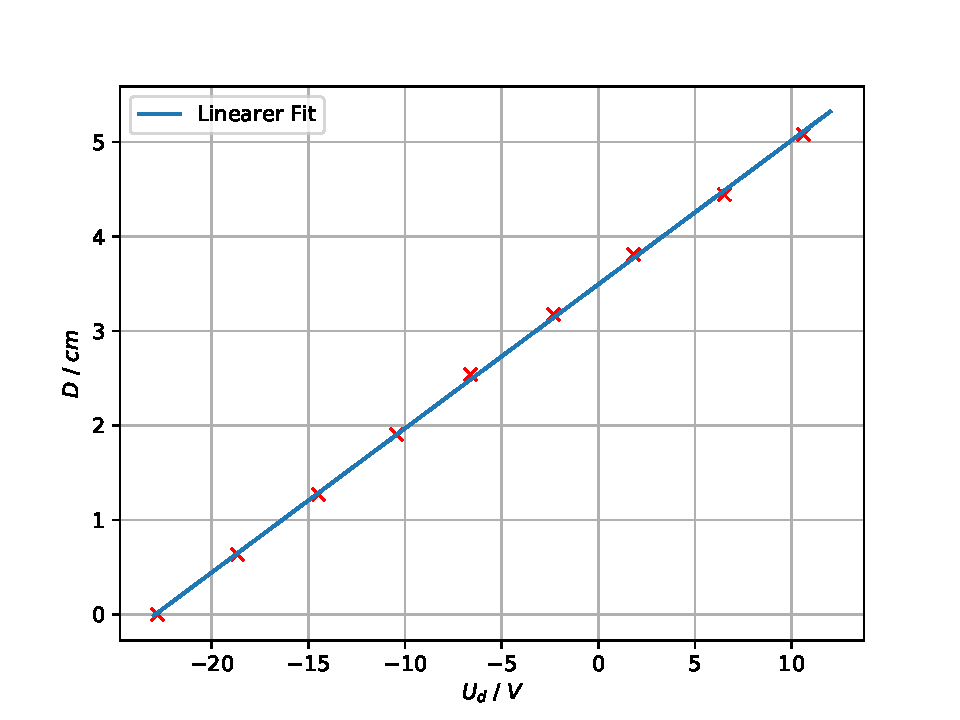
\includegraphics[width=0.7\linewidth]{../../Leuchtpunktverschiebung1}
	\caption{Die Messwerte und zugehörige Ausgleichsgerade für die Beschleunigungsspannung $U_\text{B} = \SI{220}{\volt}$.}
	\label{fig:leuchtpunktverschiebung1}
\end{figure}

\begin{figure}[h!]
	\centering
	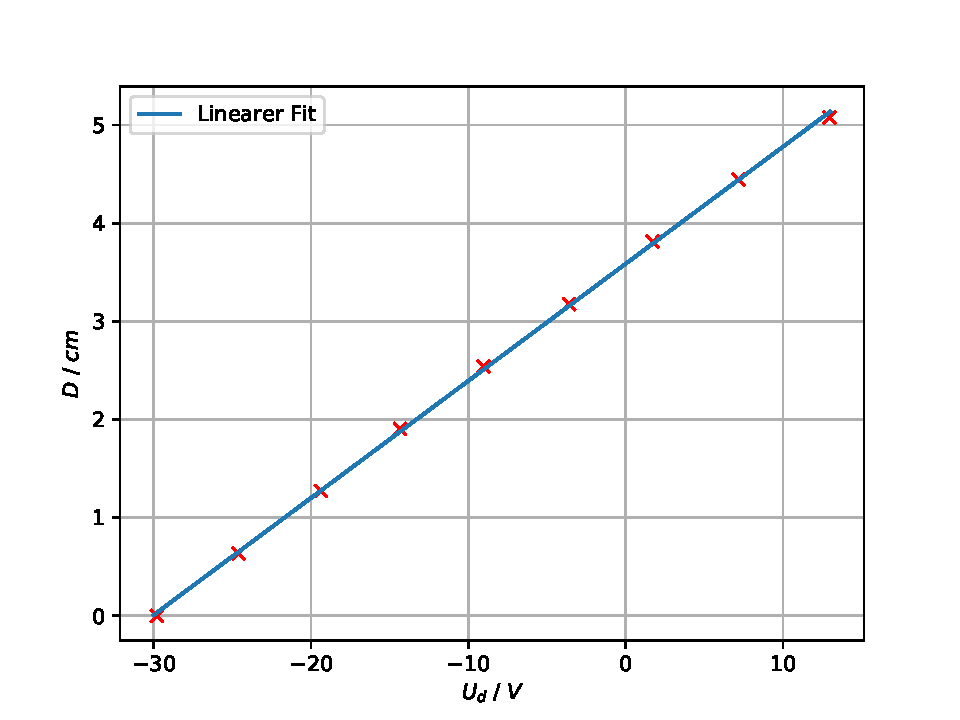
\includegraphics[width=0.7\linewidth]{../../Leuchtpunktverschiebung2}
	\caption{Die Messwerte und zugehörige Ausgleichsgerade für die Beschleunigungsspannung $U_\text{B} = \SI{300}{\volt}$.}
	\label{fig:leuchtpunktverschiebung2}
\end{figure}

\begin{figure}[h!]
	\centering
	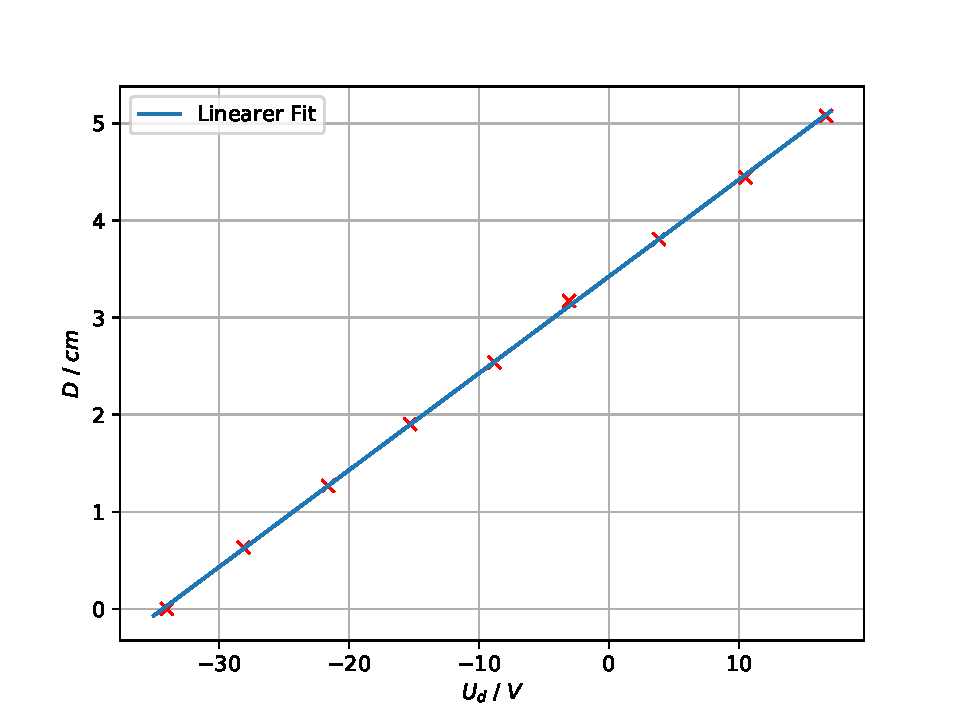
\includegraphics[width=0.7\linewidth]{../../Leuchtpunktverschiebung3}
	\caption{Die Messwerte und zugehörige Ausgleichsgerade für die Beschleunigungsspannung $U_\text{B} = \SI{350}{\volt}$.}
	\label{fig:leuchtpunktverschiebung3}
\end{figure}

\begin{figure}[h!]
	\centering
	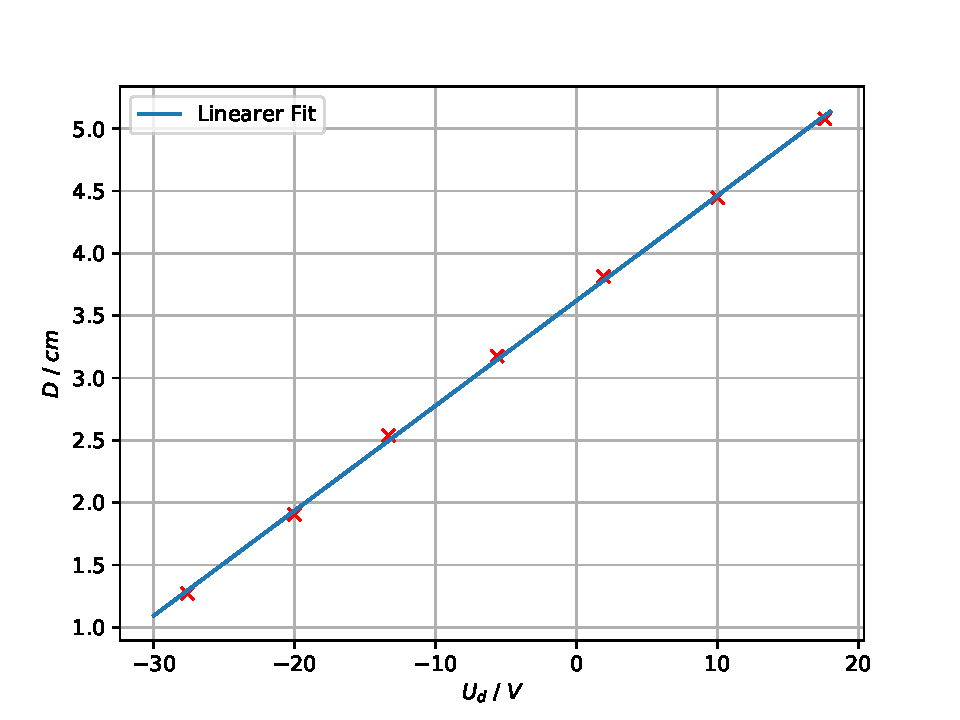
\includegraphics[width=0.7\linewidth]{../../Leuchtpunktverschiebung4}
	\caption{Die Messwerte und zugehörige Ausgleichsgerade für die Beschleunigungsspannung $U_\text{B} = \SI{420}{\volt}$.}
	\label{fig:leuchtpunktverschiebung4}
\end{figure}

\begin{figure}[h!]
	\centering
	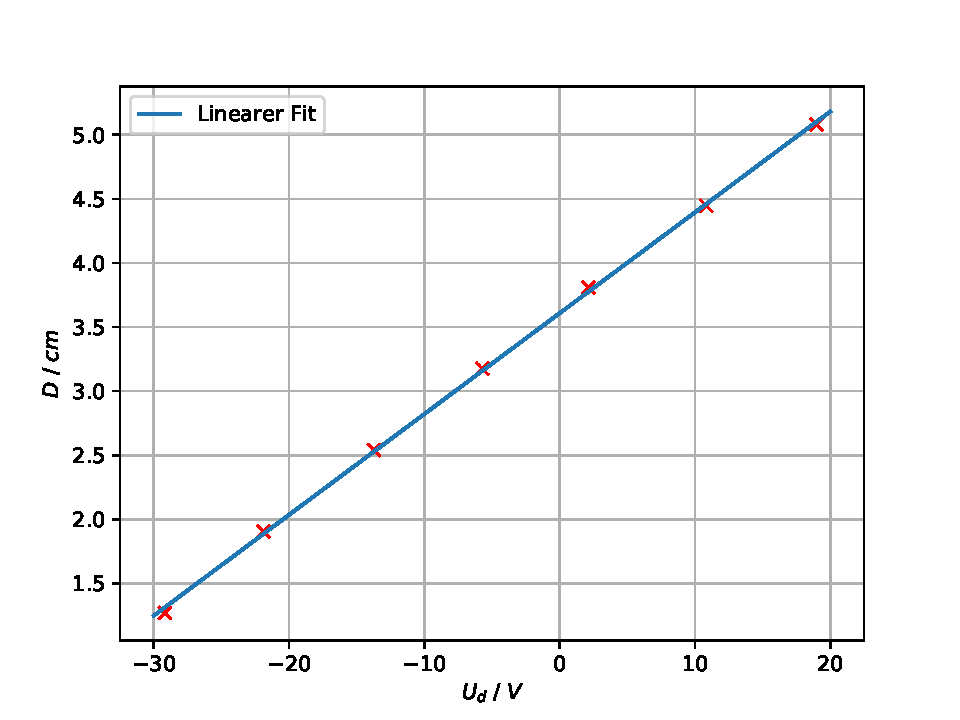
\includegraphics[width=0.7\linewidth]{../../Leuchtpunktverschiebung5}
	\caption{Die Messwerte und zugehörige Ausgleichsgerade für die Beschleunigungsspannung $U_\text{B} = \SI{450}{\volt}$.}
	\label{fig:leuchtpunktverschiebung5}
\end{figure}


\subsection{Bestimmung der Apparaturkonstante}

Als nächstes werden die errechneten Steigungen sowie die jeweiligen Fehler für einen weiteren Diagramm verwendet. Diese müssen gegen $\frac{1}{U_\text{B}}$ aufgetragen werden und erneut eine lineare Ausgleichsgerade durchgeführt. Die neuen errechnete Wertepaare werden in die Abbildung \ref{fig:apparaturkonstante} eingetragen. Die Steigung der Ausgleichsgeraden und der y-Achsenabschnitt der Form in der Gleichung \ref{eq:ausgleichsgerade} werden vom Python-Modul Scipy curve\_fit berechnet und betragen:

\begin{align*}
m &= \SI{32,004 \pm 1,396}{\cm} \\
b &= \SI{0,008 \pm 0,004}{\frac{1}{\volt}.}
\end{align*}

\begin{figure}[h!]
	\centering
	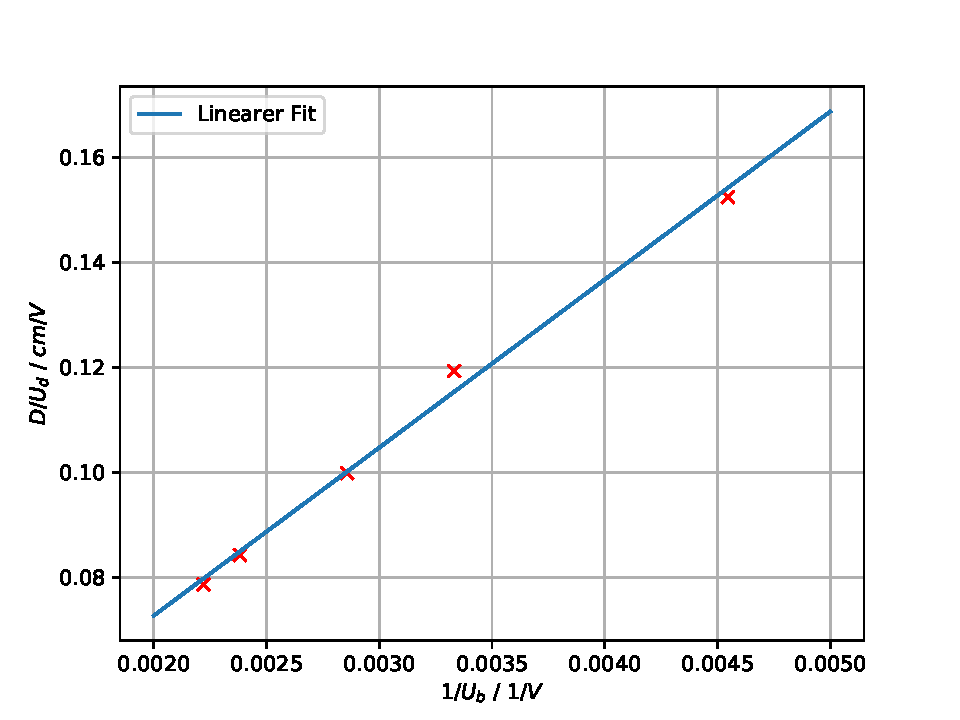
\includegraphics[width=0.7\linewidth]{../../Apparaturkonstante}
	\caption{Ausgleichsgerade für die Empfindlichkeit mit einer reziproken Beschleunigungsspannung.}
	\label{fig:apparaturkonstante}
\end{figure}

Der Mittelwert $\bar{x}$ aus $n$ Stichproben $x_{i}$ ergibt sich aus:
\newline
\begin{equation}
\bar{x}=\frac{1}{n}\sum \limits_{i=1}^n x_{i}
\label{eq:mittelwert}
\end{equation}

Das neue Ergebnis soll zunächst nun mit der Größe $\frac{pL}{2d}$ verglichen werden, wobei $p$ die Länge der Ablenkplatte, $L$ die Strecke zwischen Ablenkkondensator und Leuchtschirm und $d$ der Abstand der Kondensatorplatten sind. Diese Größe kann theoretisch durch die jeweiligen angegeben Größen aus der Konstruktionszeichnung in der Anleitung \cite[7]{anleitung501} berechnet werden. 
Die Größen aus der Konstruktionszeichnung betragen:
\begin{align*}
p &= \SI{1,9}{\cm} \\
L &= \SI{15,33}{\cm}.
\end{align*}
Dabei wird für den Abstand $d$ die zwei Werte am Anfang und am Ende der Kondensatorplatten aus der Konstruktionszeichnung übernommen:
\begin{align*}
d_1 &= \SI{0,38}{\cm} \\
d_2 &= \SI{0,95}{\cm}
\end{align*}
und der Mittelwert mittels Gleichung \ref{eq:mittelwert} bestimmt:
\begin{equation*}
d = \SI{0,665}{\cm}.
\end{equation*}

Daraus ergibt sich dann:
\begin{equation*}
\frac{pL}{2d} = \SI{21,9}{\cm}.
\end{equation*}

\subsection{Wechselstromfrequenz des Sinusgenerators}
Die Wechselstromfrequenz ist auf einen Wert zwischen $\SI{80}{\Hz}$ und $\SI{90}{\Hz}$ eingegrenzt. Für diesen Versuchsteil wird eine Beschleunigungsspannung $U_\text{B} = \SI{450}{\volt}$ verwendet. Die Amplitude der Sinuswelle beträgt $1$ Kästchen auf dem Leuchtschirm, die in der aufgenommenen Abbildung \ref{fig:3070380616627317904748572025993656149737472n} zu sehen ist. 
In der Tabelle \ref{tab:Sägezahnfreq} befinden sich die aufgeführten Frequenzen der Sägezahnspannung für eine stehende Darstellung. 

\begin{table}[htbp]
	\centering
	\caption{Messwerte für Abgleich der Sägezahnfrequenz.}
	\label{tab:Sägezahnfreq}
	\begin{tabular}{c c c}
		\toprule
	    n & $\nu / \si{\Hz}$ & $\nu \cdot n / \si{\Hz}$ \\
		\midrule
		0,5 & 160,44 & 80,22 \\
		1 & 80,2 & 80,2 \\
		2 & 40,24 & 80,24 \\
		3 & 25,03 & 75,09 \\
		\bottomrule
	\end{tabular}
\end{table}

Für die angelegte Frequenz wird mithilfe der Gleichung \ref{eq:mittelwert} den Mittelwert des Frequenz bestimmt und es ergibt sich:

\begin{equation}
\nu = \SI{78,93 \pm 0,00}{\Hz}.
\end{equation}

Zur Bestimmung des Scheitelwerts der Spannung(die maximale Amplitude) wird die Empfindlichkeit der Röhre benötigt. Diese wurde für die verwendete Spannung von $U_\text{B} = \SI{450}{\volt}$ bestimmt. Die Gesamthöhe der Kurve betrug $1$ Kästchen und somit beträgt die Amplitude:
\begin{equation}
\label{eq:amplitude}
D_\text{max} = \SI{0,635}{\cm}.
\end{equation}
Dann wird die Scheitelspannung mit Hilfe der Amplitude aus der Gleichung \ref{eq:amplitude} und der Gesamthöhe der Kurve ermittelt und beträgt:
\begin{align*}
\frac{D_\text{max}}{U_\text{sin}} = \SI{0,0786}{\volt\per\cm}\\
\Leftrightarrow U_\text{sin} = \frac{D_\text{max}}{\SI{0,0786}{\volt\per\cm}} = \SI{8,07}{\volt}.
\end{align*}

\begin{figure}[h!]
	\centering
	\includegraphics[width=0.4\linewidth]{../../30703806_1662731790474857_2025993656149737472_n}
	\caption{Die Amplitude der Sinuswelle auf dem Leuchtschirm.}
	\label{fig:3070380616627317904748572025993656149737472n}
\end{figure}

